This post hoc diagnostic was motivated by the primary failures. It uses General training data and its fixed validation target only, model seed 0, and three generated draws per probe. No new test score is obtained or used to choose a candidate. Trials are reported together rather than replacing the unsuccessful primary setting. These exploratory results do not establish cross-seed robustness.
Table~\ref{tab:stability} records the initial and final validation outcomes.
\begin{table}[t]\caption{Validation-only General optimization study. All values are means of three Monte Carlo draws from one seed-0 model, not independent training replicates. MMD columns are multiplied by $10^3$; optimizer counts include critic warmup.}\label{tab:stability}\centering\small
\begin{tabular}{@{}llrrrrr@{}}\toprule
Configuration & Generator LR & Gen./field steps & Total updates & Initial val. & Final val. & Train s \\
\midrule
Raw random MLP, C=5 & 1e-05 & 2000 & 12500 & 750.34 & 256.37 & 19.8 \\
Periodic random MLP, C=5 & 1e-05 & 2000 & 12500 & 750.34 & 292.37 & 20.6 \\
Periodic random GMM, C=5 & 1e-05 & 2000 & 12500 & 203.86 & 199.85 & 20.8 \\
Periodic train-fit GMM, C=5 & 1e-05 & 2000 & 12500 & 0.82 & 0.83 & 20.7 \\
Periodic random MLP, C=10 & 1e-05 & 2000 & 22500 & 750.34 & 298.39 & 34.9 \\
Periodic RFM & 2e-04 & 22500 & 22500 & 195.40 & 1.91 & 30.4 \\
Periodic random MLP, C=5 & 2e-04 & 10000 & 60500 & 750.34 & 34.91 & 164.3 \\
Periodic random GMM, C=5 & 2e-04 & 10000 & 60500 & 203.86 & 16.40 & 171.0 \\
Periodic random MLP, C=5 & 1e-04 & 2000 & 12500 & 750.34 & 40.23 & 20.7 \\
Periodic random MLP, C=5 & 2e-04 & 2000 & 12500 & 750.34 & 35.00 & 20.8 \\
\bottomrule\end{tabular}\end{table}
The periodic critic/field uses sine and cosine spatial harmonics 1--4, eight Fourier time frequencies, width 128, and three affine layers. The study adds 500 critic-only warmup updates, five or ten critic updates per generator iteration, and slower generator learning rates, with the higher-rate refinement recorded separately. Its flow control uses the same periodic field architecture and fixed update counts; it must not be confused with the raw-angle controlled RFM in the primary table.
Figure~\ref{fig:stability} shows illustrative configurations from this post hoc study.
\begin{figure}[t]\centering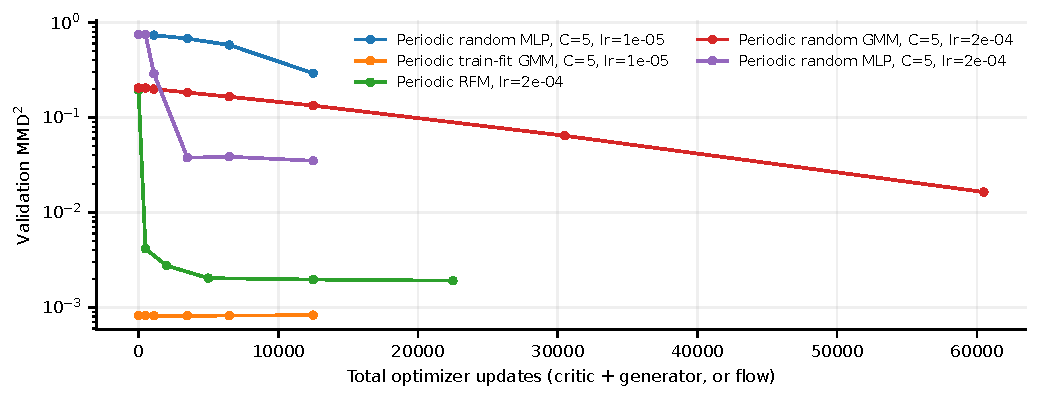
\includegraphics[width=\textwidth]{figures/validation_stability.pdf}
\caption{General validation diagnostics from one training seed. Lines join fixed probe checkpoints; they are not interpolated test estimates. Curves illustrate retention, random initialization, higher-rate refinement, and periodic RFM; all completed trial outcomes are listed in Table~\ref{tab:stability}. Update counts are not equal FLOPs; measured training times appear in the table.}\label{fig:stability}\end{figure}
